\documentclass[a4paper,11pt]{article}
\usepackage[a4paper, left=1.5cm, right=1.5cm, top=2.0cm, bottom=3.5cm, headsep=1.2cm]{geometry}
\usepackage{polski}
\usepackage{amssymb}
\usepackage[utf8]{inputenc}
\prefixing
\usepackage{latexsym}
\usepackage{graphicx}
\author{Klaudia Balcer}
\title{Raport 1 ADZD}
\frenchspacing
\begin{document}
\maketitle
\tableofcontents
\pagebreak

\section{Zadanie 1}

W tym zadaniu pokażę oszacowania ciężkości ogona rozkładu normalnego:

$$ \phi(t) \frac{t}{t^{2}+1} \leq 1  - \Phi(t) \leq \frac{\phi(t)}{t} $$

Na wykładzie uduwodniliśmy, że:

$$ \frac{\phi(t)}{t}(1-\frac{1}{t^{2}}) \leq 1  - \Phi(t) \leq \frac{\phi(t)}{t} $$

Łatwo można pokazać, że poza zbiorem skończonej miary (Lebesgue'a) zachodzi:

$$ \phi(t) \frac{t}{t^{2}+1} \leq \frac{\phi(t)}{t}(1-\frac{1}{t^{2}})$$

Powyższa nierówność może zostać przekształcona do nierówności wielomianowej (skorzystałam z tego, że gęstość rozkładu normalnego jest funkcją wszędzie dodatnią):

$$t^{4} - t^{3} -1 \geq  0 $$ 

Która jest spełniona poza odcinkiem (-0.82, 1.39)\footnote{są to przybliżenia miejsc zerowych tego wielomianu odponiednio z niedomiarem i nadmiarem.} Pokazaliśmy jednak, że nawet na odcinku (0.2, 1.39) oszacowanie to jest poprawne.

Poniższe wykresy przedstawiają poprawność tego oszacowania, a także asymptotyczną równość wszystkich trzech funckji. Pierwszy wykres korzysta wprost z wartości,  drugi natomiast z ilorazów funkcji szacowanej i szacujących. 

Szczególnie ważny jest dla nas drugi wykres. Na pierwszym widzimy, że wszystkie funkcje zbiegają do zera i poprawność oszacowania. Na drugim natomiast dodatkowo uwypukla się ważna własność oszacowania, że zbiegają do zera w bardzo podobnym tempie.  Stąd wniosek, że przedstawione oszacowania są dobre. 

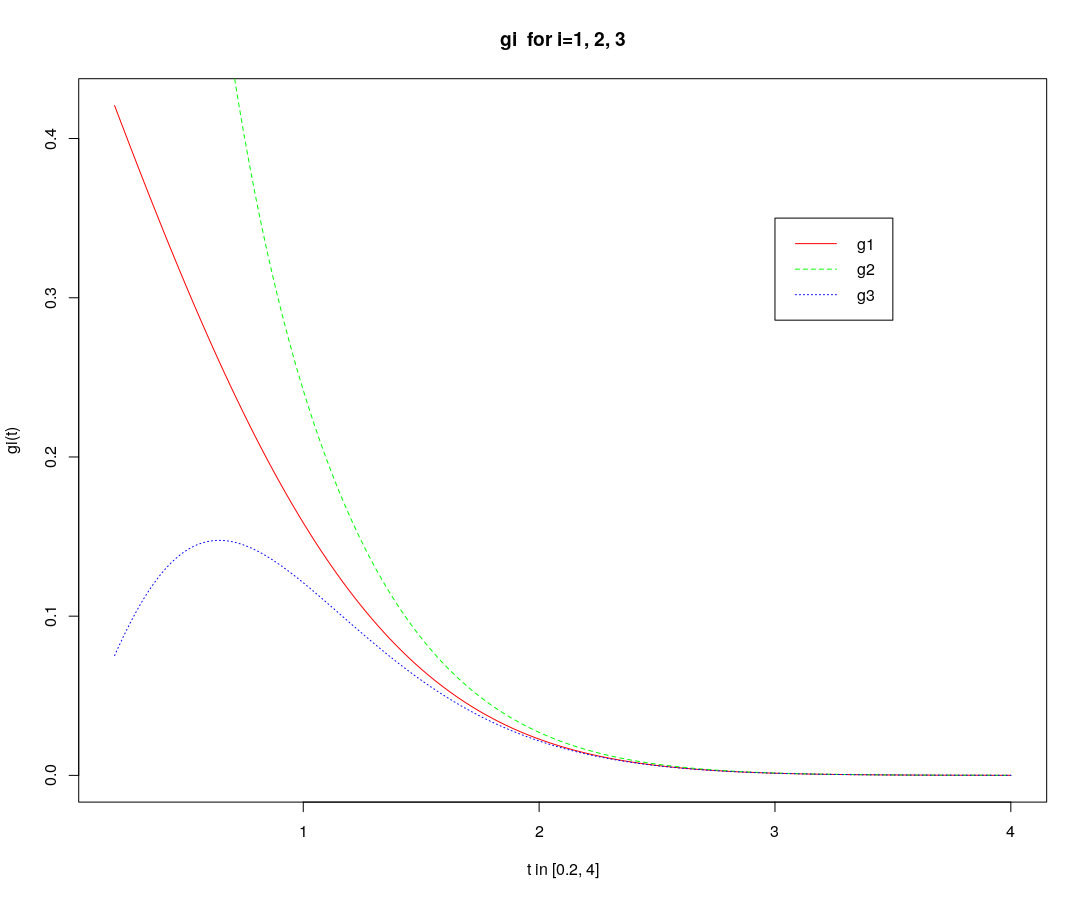
\includegraphics[scale=.3]{plot1.png} 
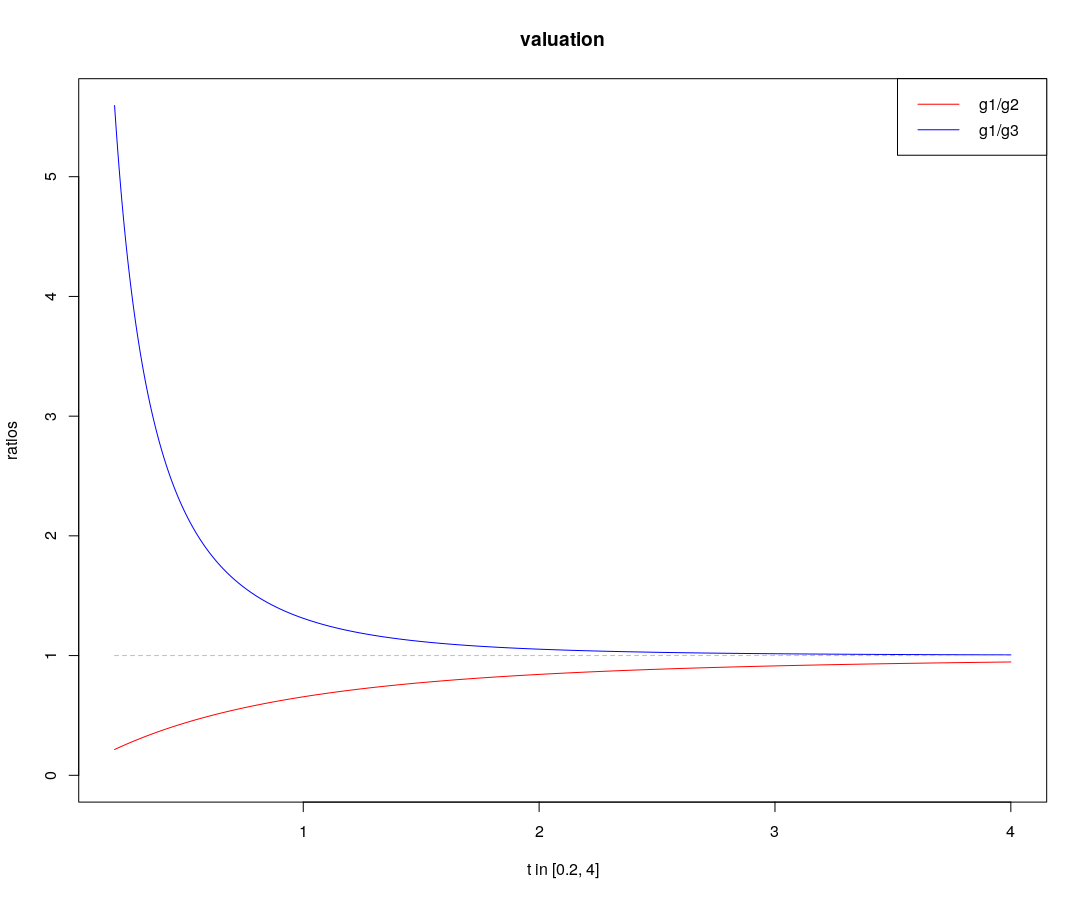
\includegraphics[scale=.3]{plot2.png} 

\pagebreak

\section{Zadanie 2}

W tym zadaniu przedstawię oszacowanie wartości krytycznej testu Bonferroniego, podanej w tym zadaniu jako $g_{1}(\alpha, p)$. Oszacujemy ją za pomocą funckji $c(p) = \sqrt{2log(p)}$ oraz  $g_{2}(\alpha, p) = \sqrt{B-log(B)}$, gdzie $B(\alpha, p) = 2log(\frac{2p}{\alpha})-log(2\pi)$. Na pierwszym wykresie widzimy, że linie ciągłą, kropkowana i przerywana się niemal nakładają - błąd bezwzględny obu oszacować jest niewielki. Drugi wykres pokazuje nam jednak jak zochowują się ilorazy funckji szacowanych i szacujących. Widzimy, że bez względu na rozmiar testu błąd względny oszacowania przez $\sqrt{2log(p)}$ jest znacznie większy niż oszacowanie wartości krytycznej testu Bonferroniego przez $g_{2}$. Wszystkie jednak błędy względne maleja wraz ze wzrostem rozmiaru próby.

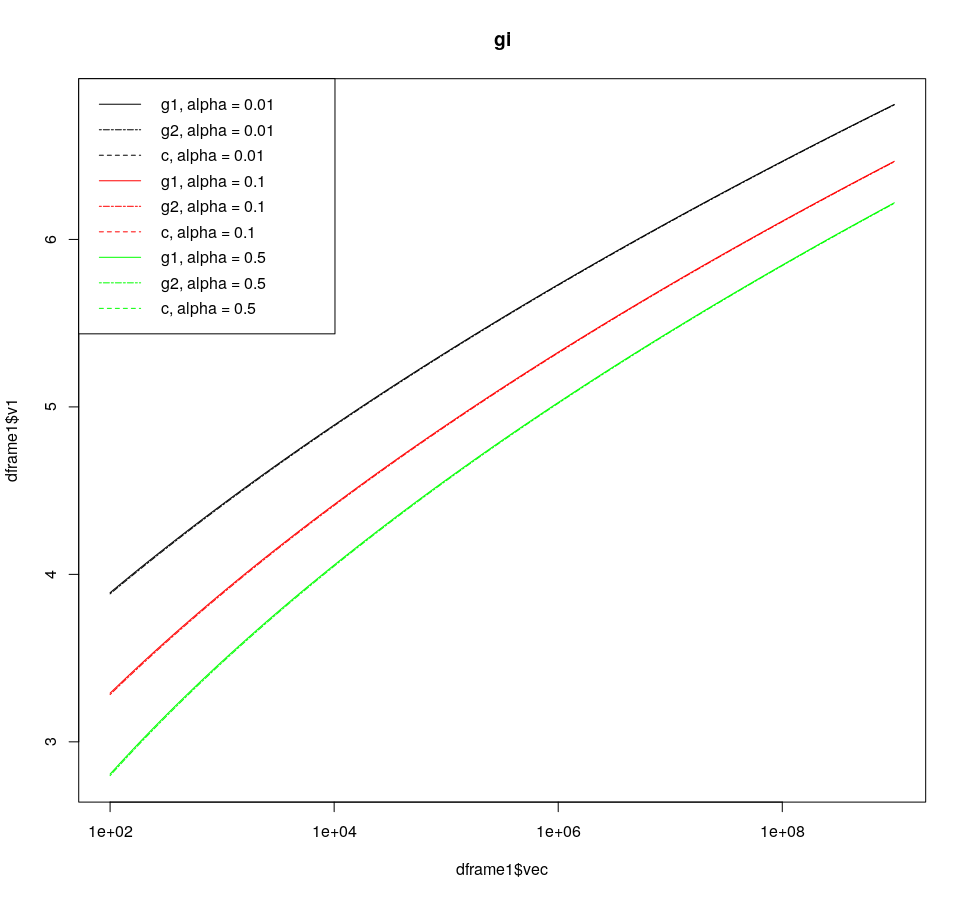
\includegraphics[scale=.3]{plot3.png} 
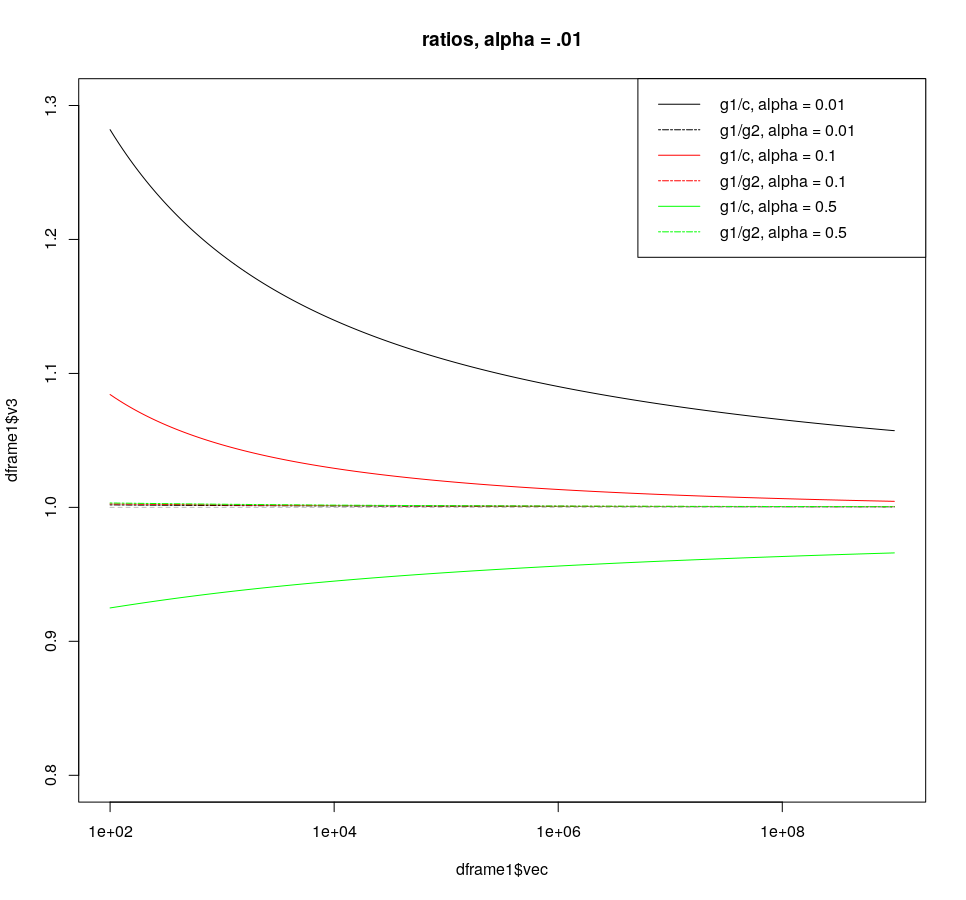
\includegraphics[scale=.3]{plot4.png}


\section{Zadanie 3}

Przedsatawię dążenie statystyki testu Bonferroniego hipotyzy globalnej do wartości krytycznej przy rosnącej liczbie zmiennych. Wykres po lewej stronie pokazuje nam wielkość statystyk testowych dla kolejnych prób (punktów trajektorii) rosnących rozmiarów w odniesieniu do oszacowania wartości krytycznej testu (badego w zadaniu 2). Większość punktów znajduje się poniżej szarej linii wskazującej wartość krytyczną. Sześć punktów powyżej szarej linii to sytuacje, kiedy popełniliśmy błąd pierwszego rodzaju - odrzucona została hipoteza zerowa, mimo że dane pochodzą z rozkładu o średniej 0. Na drugim wykresie obserwujemy stosunek wartości statytyki testowej do wartości krytycznej. Widzimy, że przy zwiększającej się wielkości próby, ten iloraz dąży do 1 - wartość statystyki testowej jest bardzo podobnego rzędu co wartość krytyczna testu.  

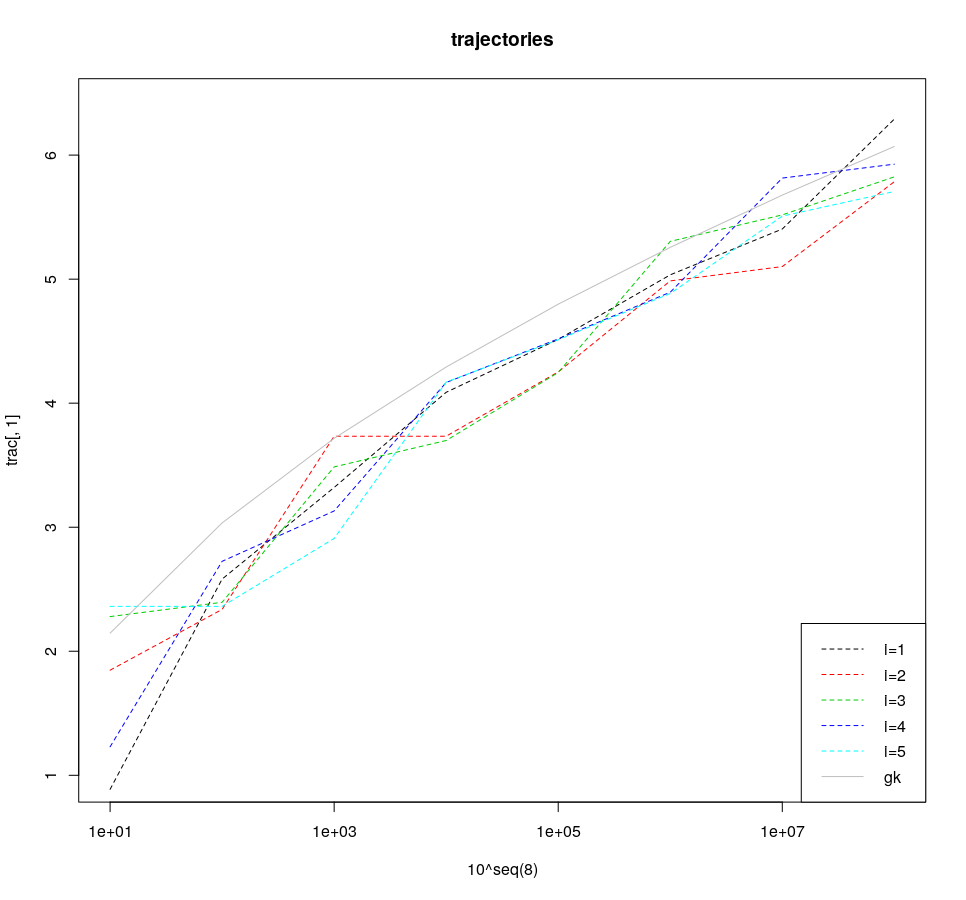
\includegraphics[scale=.3]{plot5.png} 
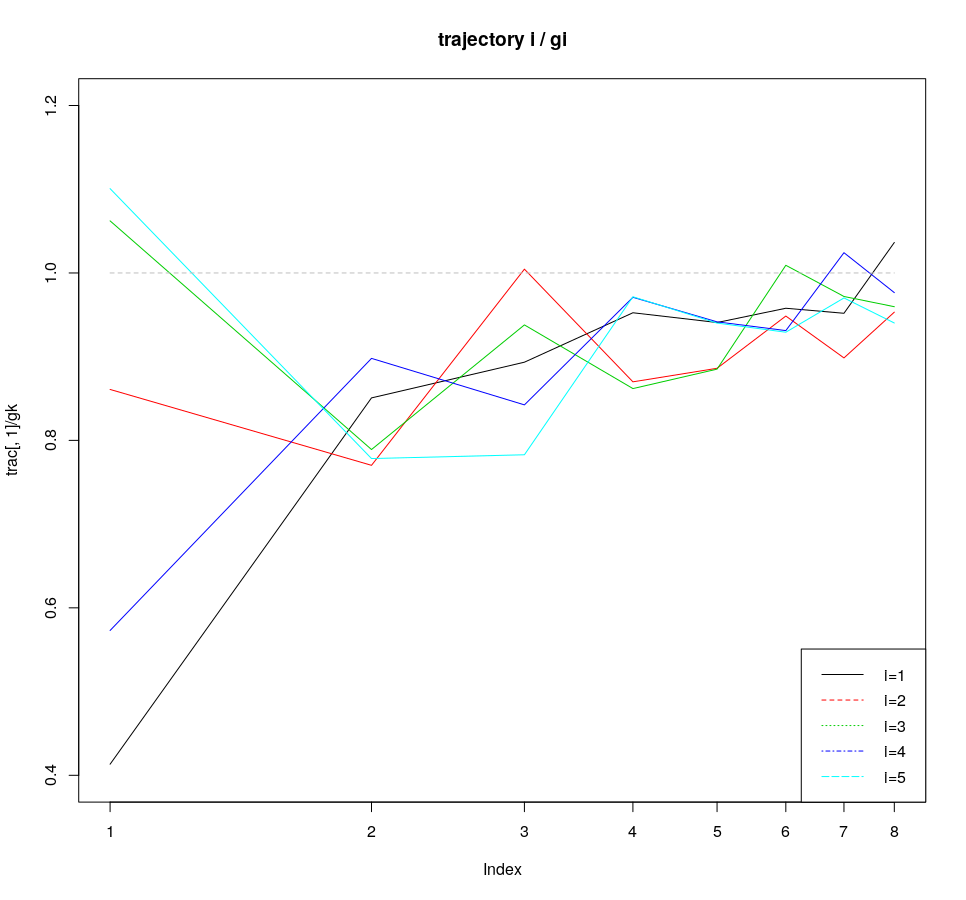
\includegraphics[scale=.3]{plot6.png}

\section{Zadanie 4}

Pokażę jak różna jest skuteczność testów Bonferroniego i $\chi^{2}$ w zależności od danych, do których je stosujemy. 

\paragraph{a} jedna długa igła:

Power of Bonferroni: 0.7274 

Power of chi-squared: 0.0812 

\paragraph{b} wiele krótkich igieł:

Power of Bonferroni: 0.1097 

Power of chi-squared: 0.9788

Zauważamy, że test Bonferroniego popełnia mniej błędów drugiego rodzaju dla silnych sygnałów (nawet  jeśli jest ich mało), natomiast test $\chi^{2}$, mimo że nie radzi sobie z wyłapywaniem pojedyńczych sygnałów, rzadziej popełnia błąd drugiego rodzaju, gdy ilość sygnałów jest duża. 

Przyczyną takiego zachowania testów jest definicja ich statystyk testowych. Bonferroni bazuje na funkcji maksimum, czyli danie mu wielu tak samo silnych sygnałów niczego nie zmienia w ich detektowalności. Natomiast test $\chi^{2}$ bazuje na sumie drugich norm zmiennych losowych. Co znaczy, że wiele małych sygnałów może był łatwiejsze do odkrycia niż silny ale pojedynczy. 

Powyższy eksperyment nie wskazuje testu generalnie lepszego. O skuteczności obu decyduje typ badanych danych. 
\end{document}